\section{Main files for technical writing report} \textit{Note:} This section contains the main information required for a technical report. The remainder of this document contains additional information which is \textit{not} required for further reports, and includes duplicate references to to files listed here. Please include:\markdownRendererInterblockSeparator
{}\markdownRendererUlBeginTight
\markdownRendererUlItem \textbf{Introduction}: all details from sec. \ref{intro}.\markdownRendererUlItemEnd 
\markdownRendererUlItem \textbf{Data source}: all details from sec. \ref{data_source}.\markdownRendererUlItemEnd 
\markdownRendererUlItem \textbf{Protocol details}: a hyperlink to the protocol source: [\href{https://github.com/DylanLawless/kit_assess/README.md}{link}].\markdownRendererUlItemEnd 
\markdownRendererUlItem \textbf{Main result}: Summary\markdownRendererUlItemEnd 
\markdownRendererUlItem \textbf{Figures}: list of figures\markdownRendererUlItemEnd 
\markdownRendererUlEndTight \markdownRendererInterblockSeparator
{}\section{Methods} \subsection{Data source} \label{data_source}\markdownRendererInterblockSeparator
{}\markdownRendererUlBeginTight
\markdownRendererUlItem Description: The sequencing group performed library preparation for two (2) samples (AH and CH) using \href{https://www.sophiagenetics.com/clinical/oncology/solid-tumors/}{Kit X}. The performance of each was assessed with several bioinformatic methods including read quality control and performance when aligning to reference genome [\href{https://github.com/DylanLawless/kit_assess}{code available here}].\markdownRendererUlItemEnd 
\markdownRendererUlItem Data source: raw sequence data was received from [\href{https://www.sophiagenetics.com}{link group and contact address}].\markdownRendererUlItemEnd 
\markdownRendererUlItem Date: 2022-02-14\markdownRendererUlItemEnd 
\markdownRendererUlItem Link to tickets where their submission was logged: [\href{https://www.sophiagenetics.com}{link}]\markdownRendererUlItemEnd 
\markdownRendererUlItem Data integrity: [\href{https://github.com/DylanLawless/kit_assess/src/metadata/raw.md5sum}{link metadata md5sum}].\markdownRendererUlItemEnd 
\markdownRendererUlEndTight \markdownRendererInterblockSeparator
{}\subsection{Configuration}\markdownRendererInterblockSeparator
{}\markdownRendererUlBeginTight
\markdownRendererUlItem Local env: macOS v11.6 \href{https://support.apple.com/macos}{software}\markdownRendererUlItemEnd 
\markdownRendererUlItem Remote env: Red Hat Enterprise Linux Server 7.6 (Maipo) \href{https://www.redhat.com/en/technologies/linux-platforms/enterprise-linux}{software}\markdownRendererUlItemEnd 
\markdownRendererUlItem compiler intel: (19.0.5 and 19.1.1) \href{https://www.intel.com/content/www/us/en/developer/tools/oneapi/commercial-base-hpc.html#gs.ppyt3x}{software}\markdownRendererUlItemEnd 
\markdownRendererUlItem R: R v4.1.0 Camp Pontanezen \href{https://www.r-project.org}{software}\markdownRendererUlItemEnd 
\markdownRendererUlItem R libraries: versions unlisted\markdownRendererUlItemEnd 
\markdownRendererUlItem fastqc: v0.11.7 \href{https://www.bioinformatics.babraham.ac.uk/projects/fastqc/}{software}\markdownRendererUlItemEnd 
\markdownRendererUlItem samtools: v1.10 \href{https://www.htslib.org}{software}\markdownRendererUlItemEnd 
\markdownRendererUlItem bwa: v0.7.17 \href{https://janis.readthedocs.io/en/latest/tools/bioinformatics/bwa/bwamem.html}{software}\markdownRendererUlItemEnd 
\markdownRendererUlItem picard: v2.20.8 \href{http://broadinstitute.github.io/picard/}{software}\markdownRendererUlItemEnd 
\markdownRendererUlEndTight \markdownRendererInterblockSeparator
{}\subsection{Data exploration} * Read counts:\markdownRendererInterblockSeparator
{}read\markdownRendererEmphasis{count.sh 3. fastQC: manual run all fastq and save to ./processed/fastqc 3. fastqcr: Assess fastqc rerpots further 4. src/target}info.sh 5. src/1.trim.sh 6. src/2.align.sh 7. src/3.sort.sh 8. src/mapping.sh\markdownRendererInterblockSeparator
{}\section{Supplemental files for intermediate report} [\href{https://github.com/DylanLawless/kit_assess/data/processed/}{link}].\markdownRendererInterblockSeparator
{}\section{Result details}\markdownRendererInterblockSeparator
{}\begin{figure}[ht] \hspace*{0cm} \begin{center} 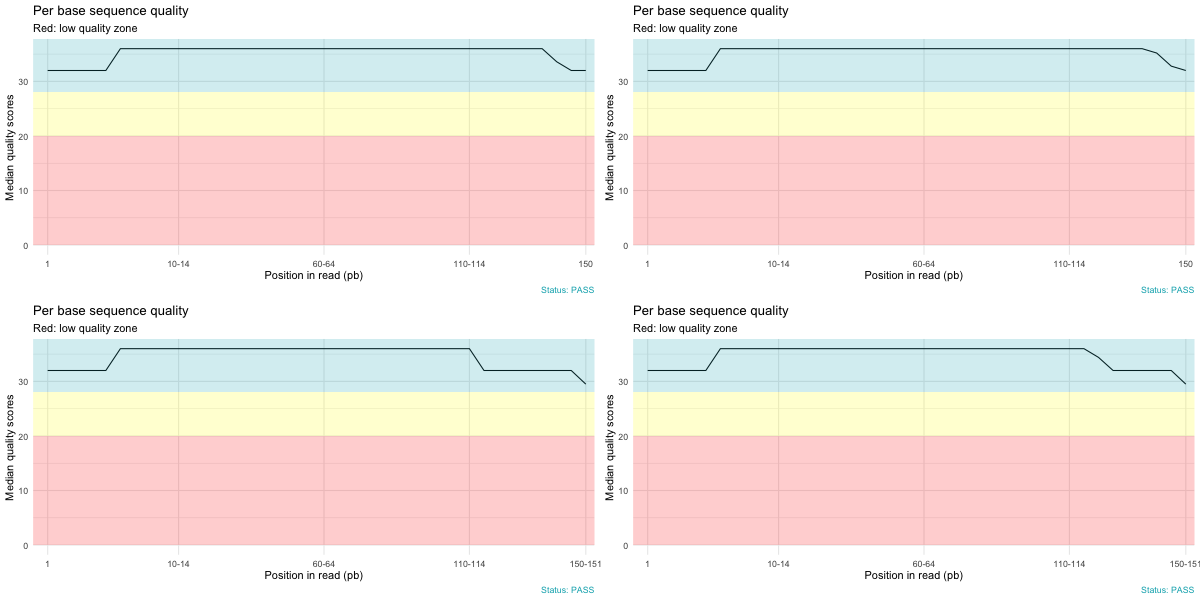
\includegraphics[scale=0.3]{p1} 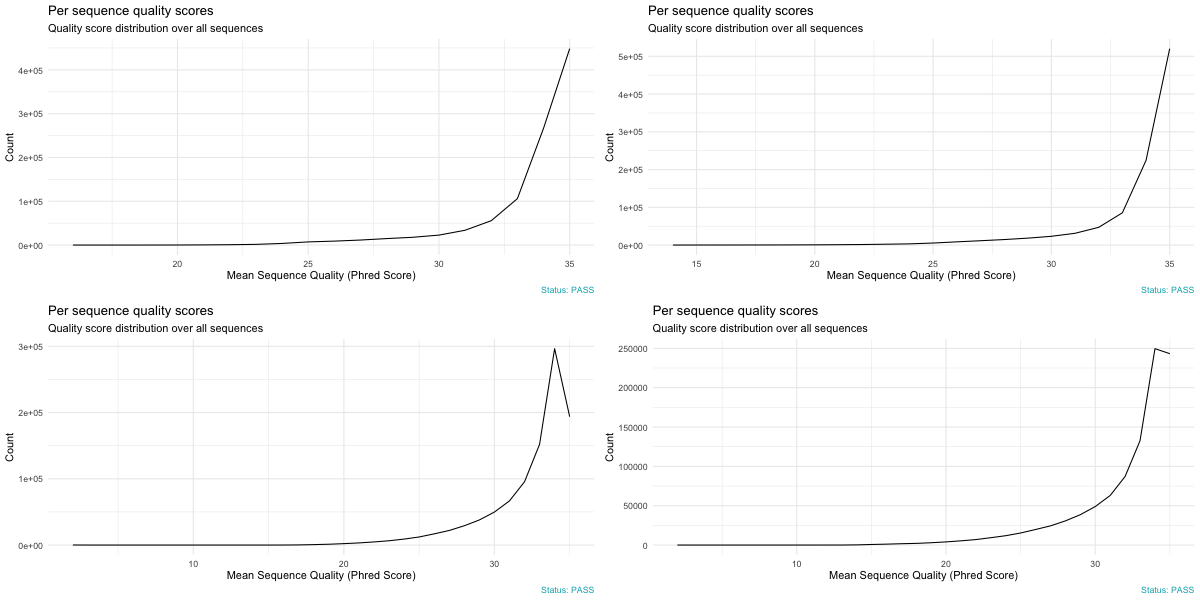
\includegraphics[scale=0.3]{p2} \caption{Caption.} \label{fig:p1p2} \end{center} \end{figure}\markdownRendererInterblockSeparator
{}\begin{figure}[ht] \hspace*{0cm} \begin{center} 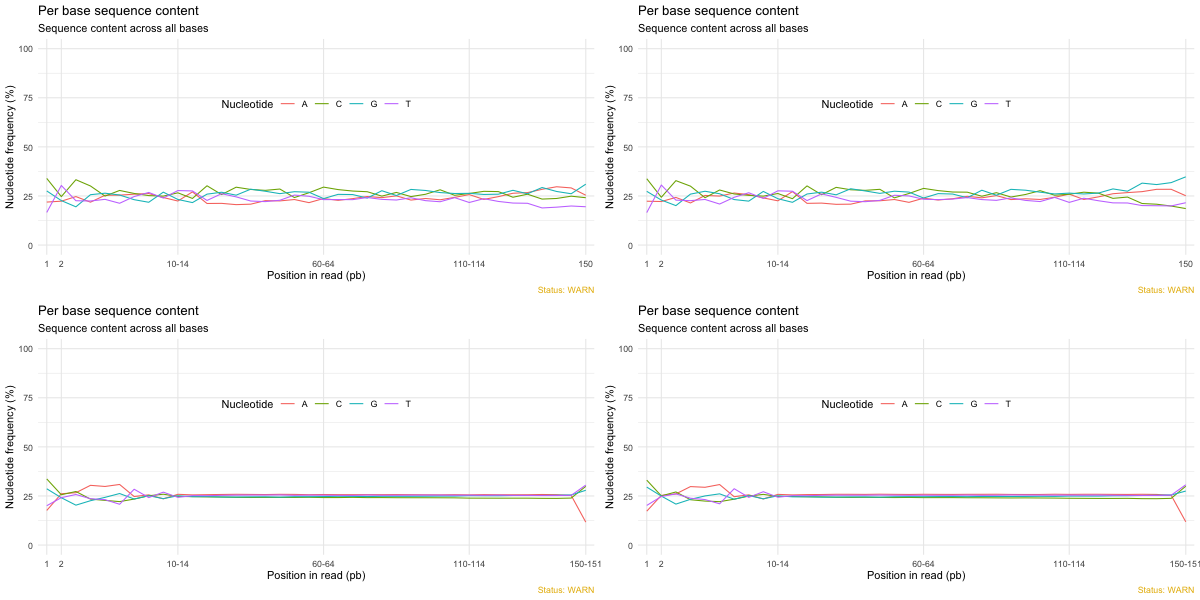
\includegraphics[scale=0.3]{p3} 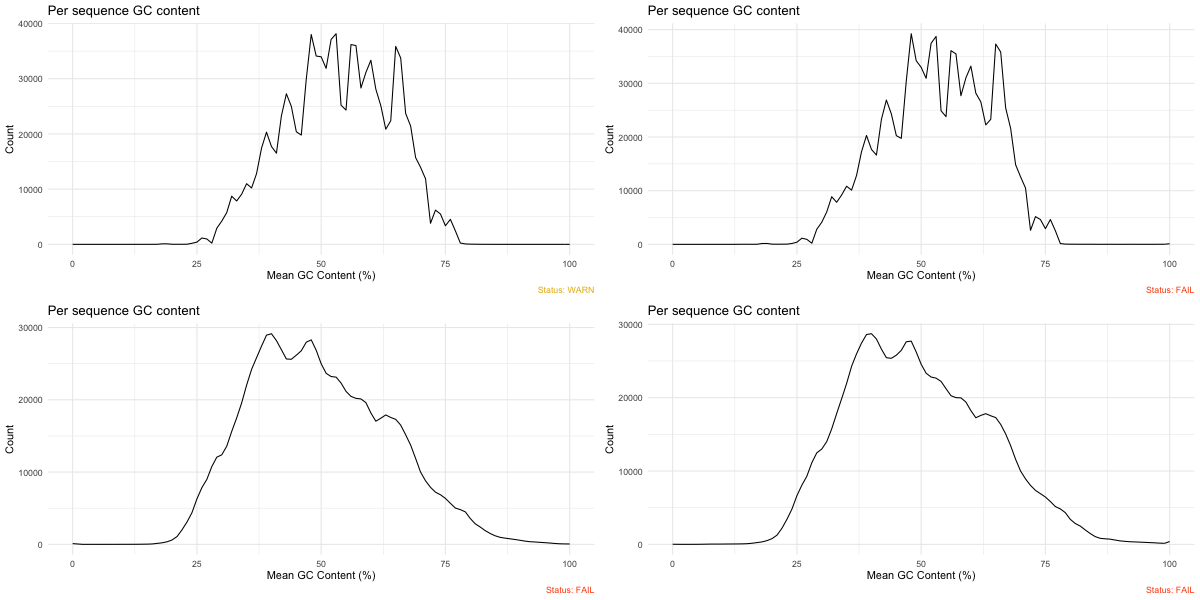
\includegraphics[scale=0.3]{p4} \caption{Caption.} \label{fig:p3p4} \end{center} \end{figure}\markdownRendererInterblockSeparator
{}\begin{figure}[ht] \hspace*{0cm} \begin{center} 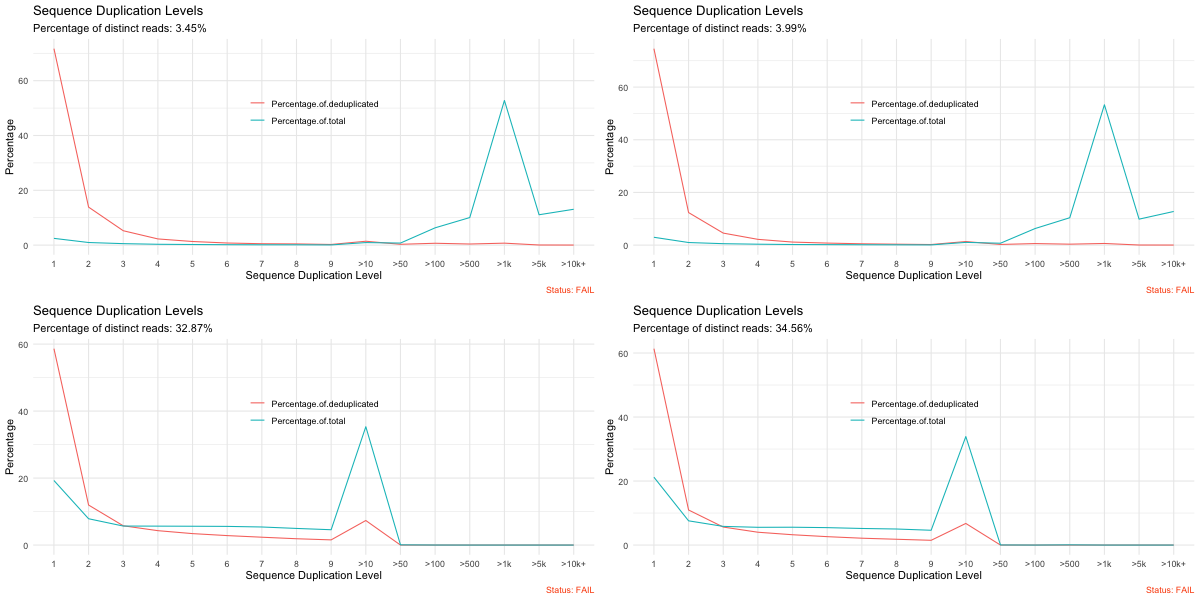
\includegraphics[scale=0.3]{p5} 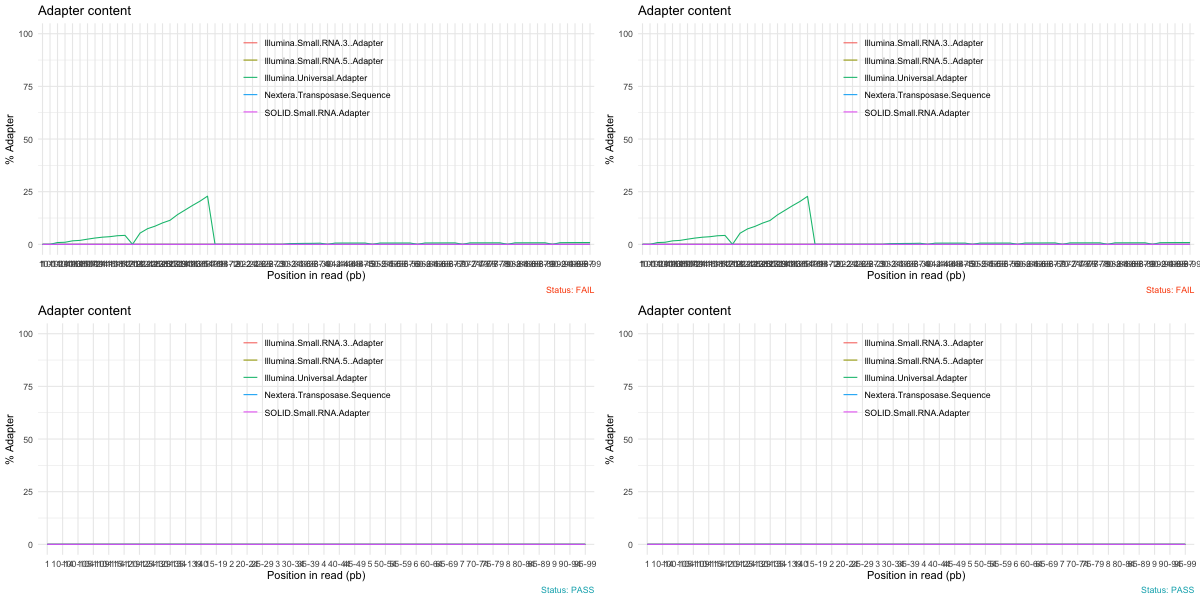
\includegraphics[scale=0.3]{p6} \caption{Caption.} \label{fig:p5p6} \end{center} \end{figure}\markdownRendererInterblockSeparator
{}\section{Methods}\relax